\section{Experiments}
\label{sec:experiments}

\noindent\textbf{Dataset}.
We perform our tests on the Dota dataset \cite{9712446}.
It contains 4677 videos taken from YouTube channels, with a resolution of $1024 \times 720$, annotated with information about the start and end of the anomaly, the category (10 in total) and the bounding boxes of the objects or persons involved.
The videos were recorded in different countries and with different light and weather conditions.
The dataset is split in approximately $70\%$ training and $30\%$ validation.
\lnote{li vogliamo ignorare o no? -> V: è un rischio perché andiamo abbastanza bene in quei casi, non saprei}
Because our benchmarks are related to the Task 1 \cite{9712446}, (online) frame-level Video Anomaly Detection, we ignore videos with unknown category or without objects, resulting in 1,305 test videos.
Furthermore, VO and OO columns are not shown because they do not contain anomalous traffic participants.

\noindent\textbf{Evaluation Metrics}.
To evaluate the performance of the models, we use the well-known Area Under Curve (AUC) metric.
This metric evaluate how well the model temporary-locate the anomaly in the videos.

\noindent\textbf{Implementation details.}
The results of the models with which we compare our model, are taken from the respective papers.
We perform the training on a single machine with 1 \lnote{XXX} GPU with \lnote{xxGB} of memory.
We use the Stochastic Gradient Descent (SGD) optimization algorithm with a learning rate of 0.0001, a \lnote{weight decay of 0.0001}, and a momentum of 0.9.

\noindent\textbf{Training details.}
Because the videos contain a non-uniform number of frames, to be able to fast training with batch-size major then one, we fixed the number of frames for each video taken into account.
In addition, we chose online the starting frame for each video for each iteration, in a way to offer to the network as diverse as possible training and reduce the effect of overfitting.
\lnote{descrivi il modello pretrained su smthv2 e saliency pretrained}

\subsection{Ablation study}

% class weight loss
% 2xsoftmax vs 1x
% learning rate differences (sto finendo l’esperimento con multipli lr)

\noindent\textbf{Short-term memory module.}

\begin{figure}[t]
\centering
	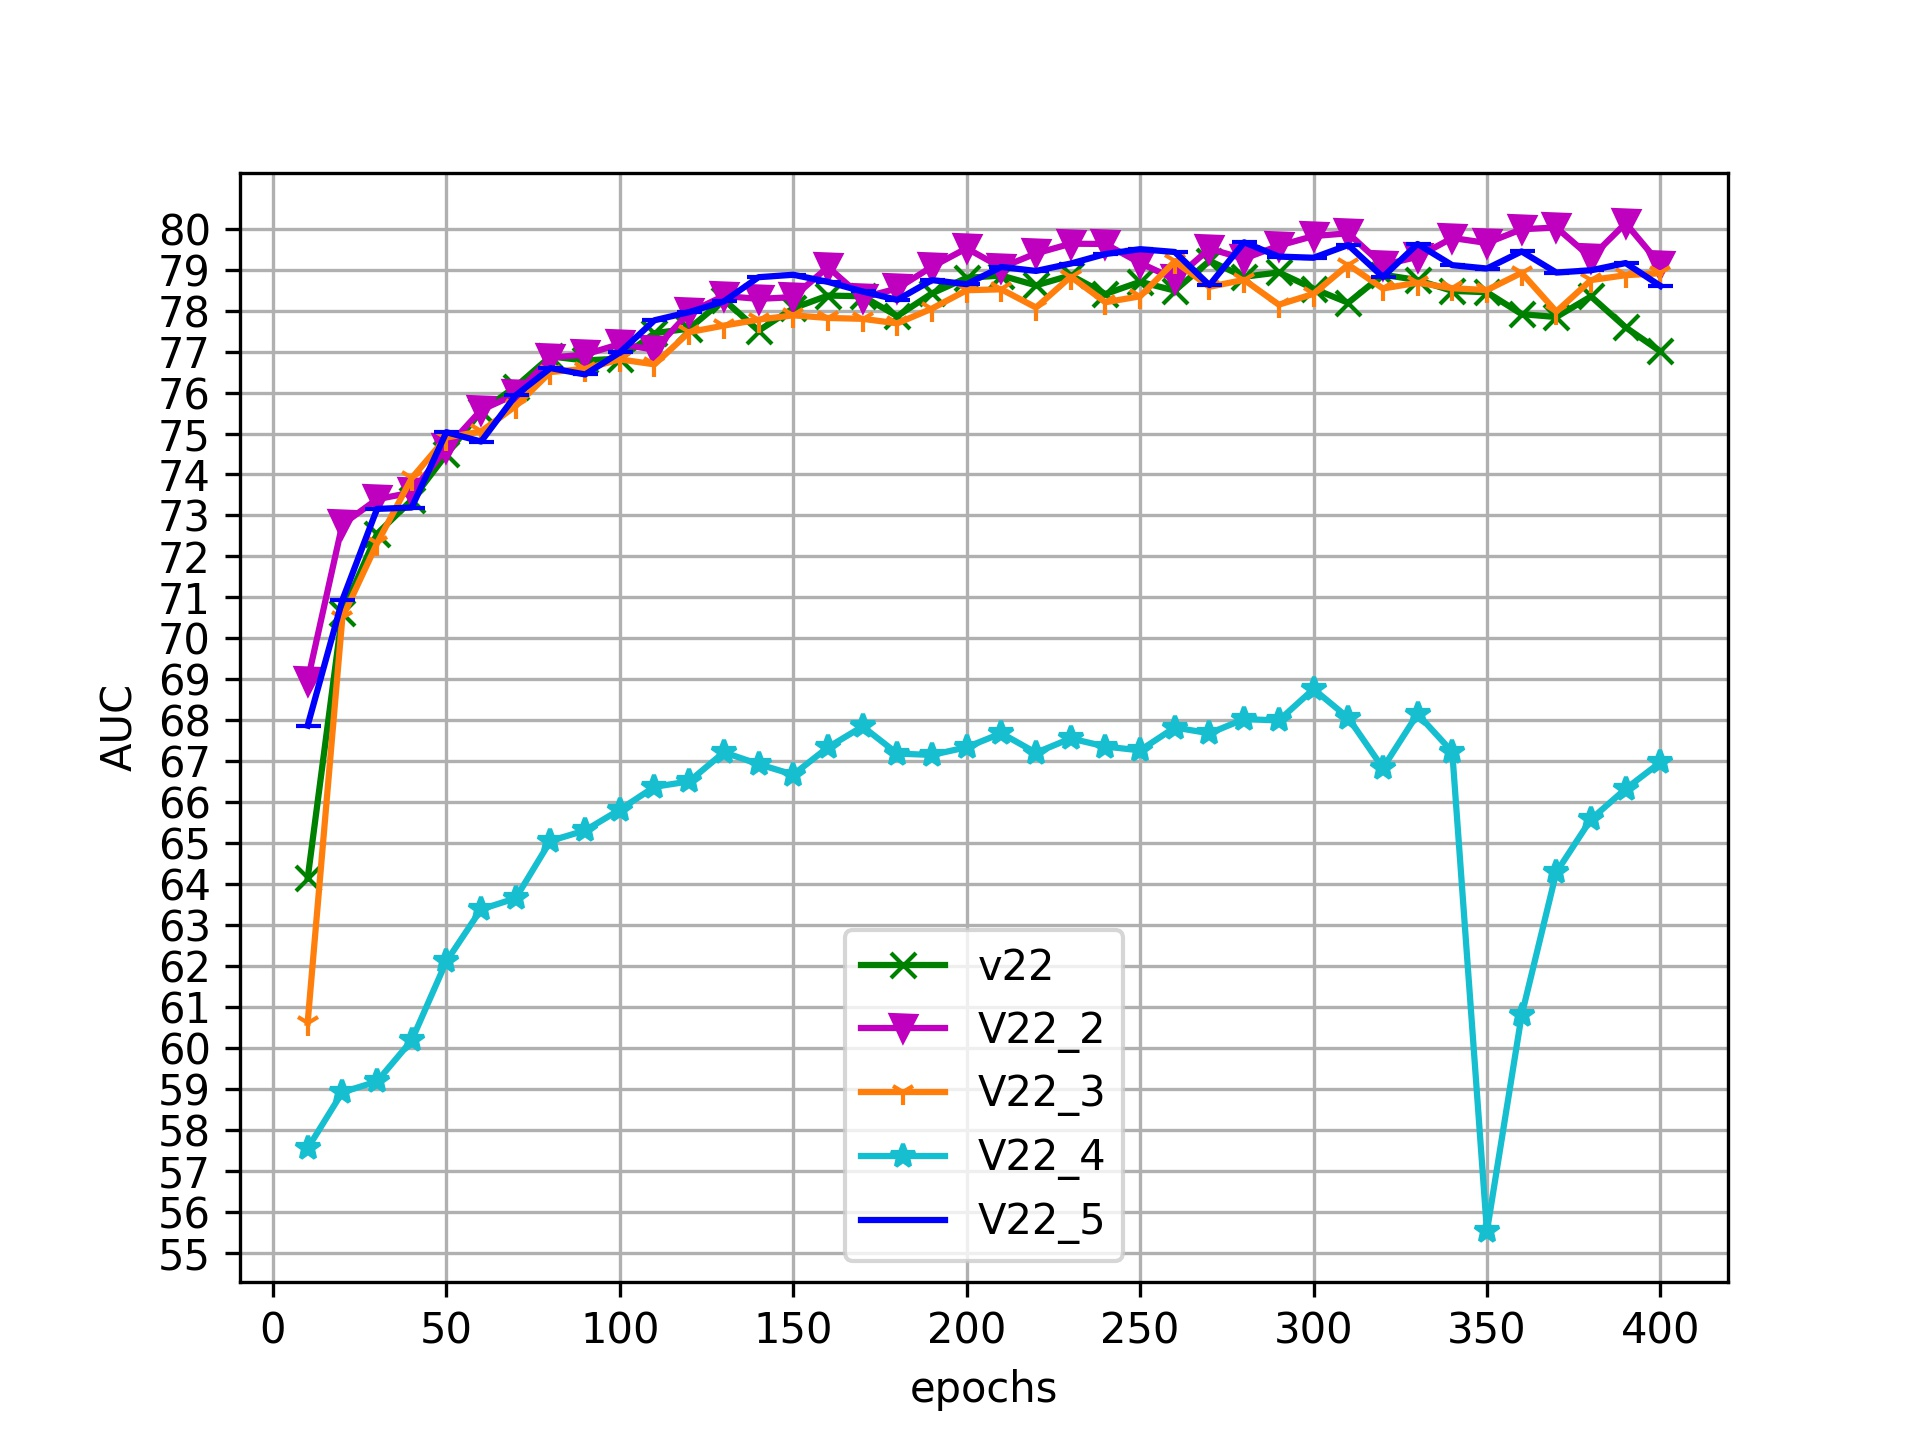
\includegraphics[trim=0 0 0 0, clip, width=1.\linewidth]{images/exp_1.jpg}
	\caption{Performance comparison changing the number of frames in input of the Short-term memory module.}
	\label{fig:bbox-iou-arch}
\end{figure}

% v22: numero di frames in input
% v23: rand frame order (v17) vs normal
% training from scratch vs pretrained (imagenet vs smth2smthv2)

\noindent\textbf{Long-term memory module.}
% posizione dell'lstm senza / prima / dopo / prim + dopo / gru
% v24, v22, v24_2: 1/2/3 # celle lstm
% v26, v26_2, v26_3: 1/2/3 # celle gru
% v27: pre + post lstm (1 cell) + saliency

\noindent\textbf{Saliency module.}
% v25, v22: con/senza/versione ridotta della saliency

\noindent\textbf{Video clip length.}
% random_batch 4/8/12/16/20/24: describi la modalità di addestramento -> per usare un batch size > 1 si è scelto di selezionare un numero max di frame da elaborare a ogni iterazione. per aggiungere diversità al training, il punto di inizio per ogni video viene scelto in modo casuale a ogni iterazione, adattando di conseguenza il ground-truth

\noindent\textbf{XXXX model}
% input shape
% versione finale vs resto del mondo su dota, and: 
%   - Phantom: https://paperswithcode.com/paper/approaches-toward-physical-and-general-video
%   - ShanghaiTech: https://paperswithcode.com/sota/anomaly-detection-on-shanghaitech
%   - CUHK Avenue: https://paperswithcode.com/sota/anomaly-detection-on-chuk-avenue
%   - UCSD Ped2: https://paperswithcode.com/sota/abnormal-event-detection-in-video-on-ucsd
